\begin{document}
\maketitle
\begin{abstract}
A noisy evaluator can preserve the ranking of every pair of tools while concealing which tool maximizes quality minus execution cost. We study stochastic Bernoulli bandits with known action prices, a shared symmetric feedback channel of unknown reliability, and optional trusted audits. We characterize exactly the decision ambiguity remaining after all proxy means are known, using a linear program with only two channel endpoints. For learning from bandit feedback, a scale-calibrated UCB algorithm separates ordinary arm exploration from a single shared calibration estimate. For two arms, channel reliability bounded below by $1/4$, price spread $D\leq1/4$, and at most $B$ expected audits, we establish the minimax execution-regret rate $\softTheta(\sqrt T+DT/\sqrt{B+1})$. When each audit costs $a\in[0,1]$, the corresponding rate is $\softTheta(\sqrt T+\min\{DT,(aD^2)^{1/3}T^{2/3}\})$. The lower bounds use environments with exactly identical free-feedback laws. Thus heterogeneous prices make an otherwise unnecessary calibration parameter statistically consequential. We also give a finite-sample decision certificate and a bound under channel misspecification. Reproducible simulations expose the calibration tradeoff and its limitations: the proved algorithm is conservative and need not outperform direct audited learning on fixed instances.
\end{abstract}
\begin{keywords}
Stochastic bandits, noisy feedback, costly observations, calibration, tool selection
\end{keywords}

\section{Introduction}
A controller choosing among software tools, model endpoints, or verification routines must compare improvements in task quality against execution prices. It may receive inexpensive automatic feedback after every action while obtaining a trusted success label only by paying for a more expensive check. An evaluator that reliably orders tools by quality is useful, but ordering alone does not determine whether a quality improvement pays for its price.

Consider two tools with prices $0$ and $0.2$. Suppose their automatic success rates are exactly $0.5$ and $0.6$. Under a symmetric evaluator with scale $\gamma=0.4$, the true success rates can be $0.5$ and $0.75$, so the expensive tool is preferable. With scale $\gamma=0.6$, the same automatic success rates correspond to true success rates $0.5$ and $2/3$, so the cheap tool is preferable. In both cases the evaluator ranks quality correctly. Even infinitely many automatic evaluations cannot reveal the optimal net-utility decision. Figure~\ref{fig:identification} depicts this ambiguity.

This issue is distinct from adversarially reversing a ranking. Under constant symmetric noise, online learning of unpriced binary rewards does not require the noise rate to be known \citep{resler2019}. The price term changes that conclusion because it is expressed in the units of the true reward and is not passed through the evaluator's channel. The relevant comparison is consequently between a noisy quality difference and a \emph{scaled} price difference. Our question is how much trusted feedback is necessary to learn that scale, and how this requirement changes as prices become more homogeneous.

We analyze a deliberately small model in which this question has a sharp answer. A trusted audit reveals the outcome of the chosen action after execution; it does not improve that outcome. The objective includes both execution regret and, when specified, audit expenditure. The shared channel makes audits transferable: the signed agreement between a trusted label and its automatic evaluation estimates the same parameter regardless of which tool was selected. The main results are the following.
\begin{enumerate}
\item An exact characterization of the residual decision problem when proxy means are known. Its minimax value is a linear program involving two channel endpoints; zero value is equivalent to a common optimal action at both endpoints (Theorem~\ref{thm:geometry}).
\item A general-$K$ upper bound separating a term of order $\softO(\sqrt{KT}/\gamma_0)$ for arm learning from a shared-calibration term of order $\softO(DT/(\gamma_0\sqrt{B+1}))$. Continued proxy feedback remains useful after the audit budget is exhausted (Theorem~\ref{thm:upper}).
\item Matching two-arm lower bounds, up to logarithmic factors, for both a hard audit budget and paid audits (Theorems~\ref{thm:budget} and~\ref{thm:price}). They quantify a continuous price-spread transition, including the audit-free equal-price case.
\item A decision certificate, a controlled misspecification bound, and an executable numerical study with retained per-seed results. These clarify the assumptions behind calibration transfer rather than asserting a general model-routing performance gain.
\end{enumerate}
The $T^{2/3}$ exponent for paid information is established in earlier work. The contribution here is its specific dependence on execution-price spread, the separation from arm exploration, and the exact residual ambiguity under a shared unknown channel. We prove sharpness for two arms; we do not claim a matching dependence on arbitrary $K$ or on vanishing $\gamma_0$.

\begin{figure}[t]
\centering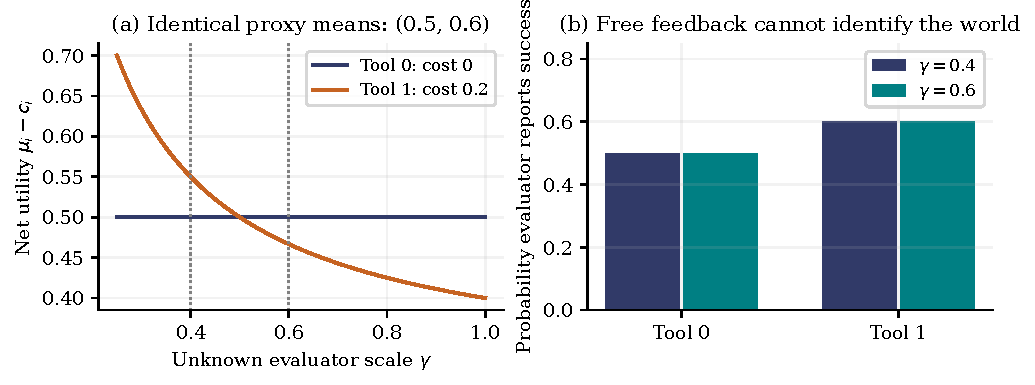
\includegraphics[width=\linewidth]{../figures/01-identification.pdf}
\caption{A quality-ranking evaluator can conceal the best priced action. Both environments have the same proxy means. The expensive tool is optimal at scale $0.4$, and the cheap tool at scale $0.6$. These are exact model quantities, not fitted experimental estimates.}\label{fig:identification}
\end{figure}

\section{Related work}
\paragraph{Transformed feedback.}
\citet{gajane2018} study bandits with known mean-corruption functions. \citet{resler2019} establish regret bounds for binary feedback passed through symmetric noise, including unknown constant noise. Our equal-price specialization inherits the ranking invariance underlying that case. We introduce a known execution-price term outside the channel and pay to recover the unknown scale. The distinction between corrupted observations and latent utility is essential; subtracting prices before applying the channel describes a different problem.

\paragraph{Paid observations and partial monitoring.}
\citet{tucker2023} establish a cube-root dependence on observation price and a $T^{2/3}$ horizon rate for costly reward observations. \citet{schur2026} develop cost-sensitive bounds and algorithms with heterogeneous observation costs and correlated actions. \citet{reyzin2026} analyze paid expert observations. We retain the ordinary feedback on unaudited rounds and distinguish execution prices $c_i$ from audit price $a$. Our calibration term disappears when the execution-price spread vanishes even if audits remain expensive. This vanishing term is not a claim to a new generic costly-observation exponent. The informative-versus-uninformative observation distinction also belongs to partial monitoring \citep{bartok2014}; our lower-bound argument is a specialization of standard information-theoretic techniques \citep{lattimore2020}.

\paragraph{Calibration, noisy labels, and surrogate rewards.}
Cost-sensitive learning with noisy labels is an established supervised-learning problem \citep{natarajan2017}. Prediction-powered inference combines predictions with trusted labels for valid inference \citep{angelopoulos2023}. \citet{ji2026} use jointly observed true and surrogate rewards in the online phase to improve bandit estimation. Cost-aware contextual routing with surrogate feedback is studied by \citet{sridhar2026}, who observe the chosen arm's true reward each round. Here true outcomes are optional and explicitly priced, and the target is a finite-horizon regret--audit frontier. \citet{ghasemi2026} use sparse audits to learn when contextual evaluators are trustworthy and show that unaudited feedback may be unidentifiable. Our evaluator is already positively informative everywhere: ambiguity arises from a shared scale and heterogeneous execution prices, not a contextual adversarial majority. None of these distinctions makes automatic evaluators universally calibratable; our shared-channel assumptions are stated next.

\section{Model and the exact no-audit decision problem}
There are $K\geq2$ actions, a horizon $T\geq K$, and known prices $c_i\in[0,1]$. Write $D=\max_i c_i-\min_i c_i$. Subtracting a common price changes neither decisions nor regret, so we take $\min_i c_i=0$. Action $i$ has unknown success probability $\mu_i\in[0,1]$ and utility $u_i=\mu_i-c_i$. At round $t$ the learner chooses action $I_t$ and audit indicator $Q_t\in\{0,1\}$ using only past information and independent internal randomness. It then draws
\begin{equation}
Y_t\sim\operatorname{Bern}(\mu_{I_t}),\qquad
F_t\sim\operatorname{Bern}((1-\gamma)/2),\qquad Z_t=Y_t\mathbin\oplus F_t,
\label{eq:channel}
\end{equation}
where $\gamma\in[\gamma_0,1]$, the lower bound $\gamma_0>0$ is known, and the fresh flip is independent of $Y_t$, the action, and the past. Success draws are fresh conditional on the action. The learner always observes $Z_t$, and observes $Y_t$ precisely when $Q_t=1$. Thus
\begin{equation}
\lambda_i:=\E[Z_t\mid I_t=i]=\frac{1-\gamma}{2}+\gamma\mu_i,
\qquad
\lambda_i-\gamma c_i=\frac{1-\gamma}{2}+\gamma u_i.
\label{eq:identity}
\end{equation}
Let $i^*\in\arg\max_i u_i$, $\Delta_i=u_{i^*}-u_i$, and $N_T=\sum_tQ_t$. Define
\begin{equation}
\Reg_T^{\rm exec}=\E\sum_{t=1}^T\Delta_{I_t},\qquad
\Reg_T^a=\Reg_T^{\rm exec}+a\E N_T.
\label{eq:regret}
\end{equation}
The comparator knows the instance, always selects an optimal action, pays its execution price, and buys no audits. An audit gives information for future decisions; its price is in the same utility units as success. No true reward is otherwise observed. The audit decision in this protocol precedes the current proxy observation, avoiding selection bias in the agreement estimate.

\subsection{All remaining ambiguity lies on a one-dimensional curve}
First suppose that the vector $\lambda$ is supplied exactly. All compatible scales form the interval
\begin{equation}
\cG(\lambda)=[g_-,1],\qquad
 g_-:=\max\{\gamma_0,\max_i|2\lambda_i-1|\},\qquad
 \mu_i(g)=\tfrac12+(\lambda_i-\tfrac12)/g.
\label{eq:compatible}
\end{equation}
This follows by imposing $0\leq\mu_i(g)\leq1$. Let $u_i(g)=\mu_i(g)-c_i$, and let $\mathcal P_K$ be the probability simplex.

\begin{theorem}[Exact ambiguity value]\label{thm:geometry}
When $\lambda$ is known and audits are prohibited, the minimax expected execution regret over compatible scales is exactly $T V(\lambda,c)$, where
\begin{equation}
\begin{split}
 V(\lambda,c)=\min_{p\in\mathcal P_K,\ v\in\R}\quad &v\\
 \text{subject to}\quad
 v&\geq u_i(g)-\sum_jp_ju_j(g)
 \quad(i\in[K],\ g\in\{g_-,1\}).
\end{split}\label{eq:lp}
\end{equation}
Moreover $V(\lambda,c)=0$ if and only if an action maximizes $\lambda_i-gc_i$ at both endpoints. Such an action is optimal throughout $\cG(\lambda)$.
\end{theorem}
\begin{proof}
Every unaudited transcript has the same distribution at every compatible $g$: action $i$ produces a Bernoulli observation with mean $\lambda_i$. Thus the average expected action frequencies $p_i=T^{-1}\E\sum_t\ind\{I_t=i\}$ do not depend on $g$, even for an adaptive policy. Its regret divided by $T$ is
$\max_i\{(\lambda_i-\sum_jp_j\lambda_j)/g-(c_i-\sum_jp_jc_j)\}$.
As a function of $1/g$ this is a maximum of affine functions, hence is convex and attains its maximum over the interval at an endpoint. Optimizing $p$ gives the lower bound in~\eqref{eq:lp}; playing an optimizer independently each round attains it. At value zero, the support of $p$ must consist entirely of maximizers at each endpoint, so it contains a common maximizer. Conversely, a common maximizer has zero regret. Each pairwise score difference is affine in $g$, establishing optimality between endpoints.
\end{proof}
For two arms whose optimal actions differ at the endpoints, let $b_-$ and $b_+$ denote the positive utility gaps there. Then
\begin{equation}
V=\frac{b_-b_+}{b_-+b_+}.
\label{eq:twoarmvalue}
\end{equation}
Indeed, mixing between the two actions equalizes their endpoint regrets. A zero intersection of optimal-action sets therefore creates irreducible linear regret, even with perfect knowledge of all proxy means. Equal prices always admit a common maximizer, so their remaining difficulty is ordinary arm learning.

\section{Learning with a shared calibration estimate}
An audited pair provides $W_t=2\ind\{Y_t=Z_t\}-1\in\{-1,1\}$ with
\begin{equation}
\E[W_t\mid I_t,\text{past},Q_t=1]=\gamma.
\label{eq:agreement}
\end{equation}
The distribution is independent of $\mu_{I_t}$. Hence audits gathered while exploiting one action still calibrate all actions. Estimating a separate correction for each arm would discard this structure.

Fix an audit budget $n\in\{0,\ldots,T\}$ and failure probability $\delta\in(0,1)$. Set $L=\log(4(K+1)T/\delta)$. Audit the first $n$ rounds. Before round $t$, let $M_t=\min\{n,t-1\}$, let $N_i(t)$ and $\widehat\lambda_i(t)$ be the count and empirical proxy mean of arm $i$, and define
\begin{equation}
\widehat\gamma_t=\begin{cases}
\gamma_0,&M_t=0,\\
\clip_{[\gamma_0,1]}\left(M_t^{-1}\sum_{s<t:Q_s=1}W_s\right),&M_t>0.
\end{cases}\label{eq:scaleestimate}
\end{equation}
After selecting each action once, \SC\ chooses
\begin{equation}
I_t\in\arg\max_i\left\{\widehat\lambda_i(t)+\sqrt{\frac{L}{2N_i(t)}}-\widehat\gamma_t c_i\right\}.
\label{eq:index}
\end{equation}
The name abbreviates scale-calibrated UCB; its exploration term is the standard Hoeffding-UCB construction \citep{auer2002}. The estimate freezes after the $n$th audit, but arm learning continues for the full horizon.

\begin{algorithm}[t]
\caption{\SC\ with a prefix audit budget}\label{alg:sc}
\begin{tabular}{@{}p{\linewidth}@{}}
\textbf{Input:} Prices $c$, horizon $T$, budget $n$, lower scale $\gamma_0$, confidence $\delta$.\\[2pt]
\textbf{Initialize:} Per-arm proxy counts and sums, and signed-agreement sum, to zero.\\[2pt]
\textbf{For} $t=1,\ldots,T$:\\
\quad 1. Select action $t$ if $t\leq K$; otherwise maximize~\eqref{eq:index}.\\
\quad 2. Set $Q_t=\ind\{t\leq n\}$ before observing current feedback.\\
\quad 3. Execute $I_t$; observe $Z_t$ and update its proxy count and sum.\\
\quad 4. If $Q_t=1$, observe $Y_t$ and add $2\ind\{Y_t=Z_t\}-1$ to the agreement sum.
\end{tabular}
\end{algorithm}

\begin{theorem}[Finite-horizon upper bound]\label{thm:upper}
Let $S_0=T$ and, for $1\leq n\leq T$, let
$S_n=1+2T\sqrt{2L/n}$. In the model~\eqref{eq:channel}, \SC\ satisfies
\begin{equation}
\Reg_T^a\leq
\frac{2K+2\sqrt{2KTL}+DS_n}{\gamma_0}
+an+\delta(1+D)T.
\label{eq:upper}
\end{equation}
Exactly $n$ audits are performed. If $\gamma$ is known, replacing $\widehat\gamma_t$ by $\gamma$ removes $DS_n$ and requires no audits.
\end{theorem}
\begin{proof}
Couple each arm to an infinite independent proxy sequence. Hoeffding's inequality and a union bound over arms and sample counts $1,\ldots,T$ give, simultaneously,
$|\widehat\lambda_i-\lambda_i|\leq r_i:=\sqrt{L/(2N_i)}$.
The signed-agreement sequence has mean $\gamma$ and range length two, so its prefix averages satisfy
$|\widehat\gamma_t-\gamma|\leq e_{M_t}$,
where $e_0=1$ and $e_m=\min\{1,\sqrt{2L/m}\}$ for $m>0$. Projection cannot enlarge the error. The joint event has probability at least $1-\delta$; independence between the two estimates is unnecessary.

On this event and after initialization, maximizing~\eqref{eq:index} yields
\begin{align}
\gamma\Delta_{I_t}
&=(\lambda_{i^*}-\gamma c_{i^*})-(\lambda_{I_t}-\gamma c_{I_t})\nonumber\\
&\leq 2r_{I_t}+(\widehat\gamma_t-\gamma)(c_{i^*}-c_{I_t})
\leq2r_{I_t}+D e_{M_t}.
\label{eq:one-step}
\end{align}
Each initialization round has regret at most $1+D\leq2$; bounding its scaled regret by $2$ is valid because $\gamma\leq1$. Summing the radii, using $\sum_{m=1}^{q}m^{-1/2}\leq2\sqrt q$ and Cauchy--Schwarz, gives $\sum_{t>K}2r_{I_t}\leq2\sqrt{2KTL}$. For $n>0$,
\begin{equation}
\sum_{t=1}^Te_{M_t}
\leq1+\sqrt{2L}\left(2\sqrt n+\frac{T-n}{\sqrt n}\right)
\leq1+2T\sqrt{2L/n}.
\label{eq:sumscale}
\end{equation}
For $n=0$ the sum is at most $T$. Divide by $\gamma\geq\gamma_0$, add $an$, and bound the execution regret on the failure event by $(1+D)T$.
\end{proof}
The calibration term has no extra factor of $K$. This is an upper-bound separation, not a claim that the full regret is independent of the number of actions. A horizon-free variant can restart on doubling epochs, at the cost of logarithmic factors; the stated algorithm and experiments use the supplied horizon.

\section{Audit budgets and prices: matching two-arm lower bounds}
Fix $\gamma_0=1/4$, prices $(0,D)$, and $0\leq D\leq1/4$. Let $\cM_D$ be the class of all two-arm instances satisfying these restrictions. For $B\in[0,T]$, the budget-constrained minimax execution regret is
\begin{equation}
\mathfrak R_T(B,D)=
\inf_{\pi:\ \sup_{\nu\in\cM_D}\E_\nu N_T\leq B}
\ \sup_{\nu\in\cM_D}\Reg_T^{\rm exec}(\pi,\nu).
\label{eq:budgetdef}
\end{equation}
The expectation constraint allows adaptive, randomized audit schedules. For the paid-audit objective define
\[\mathfrak R_T^a(D)=\inf_\pi\sup_{\nu\in\cM_D}\Reg_T^a(\pi,\nu).\] All constants below are universal; logarithmic notation suppresses factors in $T$ only.

\begin{theorem}[Budget frontier]\label{thm:budget}
For $T\geq2$ and $B\in[0,T]$,
\begin{equation}
\mathfrak R_T(B,D)=\softTheta\left(\sqrt T+\frac{DT}{\sqrt{B+1}}\right).
\label{eq:budgetrate}
\end{equation}
The lower bound holds even when the learner is told that the two proxy means are $(1/2,1/2+D/2)$ for its calibration component.
\end{theorem}
\begin{theorem}[Price frontier]\label{thm:price}
For $a\in[0,1]$,
\begin{equation}
\mathfrak R_T^a(D)=\softTheta\left(
\sqrt T+\min\left\{DT,(aD^2)^{1/3}T^{2/3}\right\}\right).
\label{eq:pricerate}
\end{equation}
At $a=0$ this is $\softTheta(\sqrt T)$. At $D=0$ audits are unnecessary for the same rate, regardless of $a$.
\end{theorem}
These statements are uniform as $D$ approaches zero. With fixed positive $a,D$, the second term eventually gives the familiar $T^{2/3}$ order. The additional $D^{2/3}$ factor and its truncation at $DT$ distinguish the calibration problem from a model with no free feedback. Figure~\ref{fig:rates} shows the rate expressions, without suggesting tight numerical constants.

\subsection{Two worlds that free feedback cannot distinguish}
For $0<h\leq1/8$ and $s\in\{-1,+1\}$, construct
\begin{equation}
\gamma_s=\tfrac12+sh,\quad
\mu_{0,s}=\tfrac12,\quad
\mu_{1,s}=\tfrac12+\frac{D}{2\gamma_s},\quad
(c_0,c_1)=(0,D).
\label{eq:hardpair}
\end{equation}
All means lie in $[1/2,5/6]$. In both worlds,
\begin{equation}
(\lambda_0,\lambda_1)=(\tfrac12,\tfrac12+\tfrac D2),\qquad
u_{1,s}-u_{0,s}=-\frac{sDh}{\gamma_s}.
\label{eq:hardgap}
\end{equation}
The optimal action is 1 in world $-$ and 0 in world $+$ when $D>0$, with each nonzero gap at least $8Dh/5$.

\begin{lemma}[Audit information]\label{lem:kl}
Let $P_-,P_+$ be the distributions of the learner's complete observable transcript in the worlds~\eqref{eq:hardpair}. For every admissible policy,
\begin{equation}
\KL(P_-\Vert P_+)\leq16h^2\E_-N_T.
\label{eq:transcriptkl}
\end{equation}
\end{lemma}
\begin{proof}
An unaudited observation has the identical Bernoulli law in both worlds. On an audited round the pair $(Y,Z)$ is equivalent to $(Y,W)$, where $Y$ and $W$ are independent. Thus its KL divergence is the sum of two Bernoulli divergences. The success-mean difference for arm 1 is
$Dh/(\gamma_-\gamma_+)\leq16h/15$, and is zero for arm 0. The success probabilities lie in $[1/2,5/6]$, and the agreement probabilities lie in $[11/16,13/16]$ with difference $h$. Using $\kl(p,q)\leq(p-q)^2/[q(1-q)]$, the KL of either arm's audited pair is at most
\begin{equation}
\left(\frac{36}{5}\frac{256}{225}+\frac{256}{39}\right)h^2<16h^2.
\label{eq:klconstant}
\end{equation}
The chain rule for KL sums this quantity only on audited rounds. The policy's action and audit kernels, conditional on the same history, are identical across worlds and contribute no divergence.
\end{proof}

\subsection{Proofs of the frontiers}
\begin{proof}[Proof of Theorem~\ref{thm:budget}]
For the upper bound, use Theorem~\ref{thm:upper} with $n=\lfloor B\rfloor$, $a=0$, and $\delta=T^{-2}$. For $B<1$, take no audits. These choices give the displayed rate since $\lfloor B\rfloor\geq(B+1)/3$ for $B\geq1$.

For the calibration lower bound, choose $h=1/(8\sqrt{B+1})$ in~\eqref{eq:hardpair}. By Lemma~\ref{lem:kl}, the transcript KL is at most $1/4$. Therefore $\TV(P_-,P_+)\leq1/2$ by Pinsker's inequality. For each $t$,
$\Pp_-(I_t=0)+\Pp_+(I_t=1)\geq1-\TV(P_-,P_+)\geq1/2$.
Consequently the larger execution regret is at least
$\frac12\cdot\frac{8Dh}{5}\cdot\frac T2=DT/(20\sqrt{B+1})$.

For the ordinary arm-learning lower bound, give the learner the channel $\gamma=1$ and set $\mu_0=1/2$, $\mu_1=1/2+D\pm\epsilon$, with $\epsilon=1/(16\sqrt T)$. Auditing reveals nothing additional. Both means are valid, the optimal actions differ with gap $\epsilon$, and the transcript KL is at most $T(256/7)\epsilon^2=1/7$. The same testing argument yields execution regret at least $\epsilon T/4=\sqrt T/64$ on one instance. Taking the larger of these two lower bounds is at least half their sum.
\end{proof}

\begin{proof}[Proof of Theorem~\ref{thm:price}]
The ordinary $\sqrt T$ lower bound still applies. For $aD>0$, fix any policy and any $h\in(0,1/8]$. If $\E_-N_T>1/(32h^2)$, its regret in world $-$ exceeds $a/(32h^2)$. Otherwise Lemma~\ref{lem:kl} and Pinsker give total variation at most $1/2$, and the previous testing argument gives maximum regret at least $2DhT/5$. Thus
\begin{equation}
\max_s\Reg_T^a(\pi,\nu_s)\geq
\min\{a/(32h^2),\ 2DhT/5\}.
\label{eq:twocases}
\end{equation}
Choose $h=\min\{1/8,(a/(32DT))^{1/3}\}$. Equation~\eqref{eq:twocases} is at least
$\frac1{20}\min\{DT,(aD^2)^{1/3}T^{2/3}\}$.

For the upper bound compare the no-audit policy with Theorem~\ref{thm:upper} using
\[n=\min\{T,\lceil(DT/a)^{2/3}\rceil\},\qquad\delta=T^{-2}.\] If the ceiling does not reach $T$, both $an$ and $DT/\sqrt n$ are bounded by the cube-root term plus a constant, up to the theorem's logarithm. If it reaches $T$ because $(DT/a)^{2/3}>T-1$, then $aT\leq D T^2/(T-1)^{3/2}=O(\sqrt T)$, since $D\leq1/4$ and $T\geq2$, and the calibration term is $\softO(D\sqrt T)$. Taking the smaller bound proves the claim. For $a=0$, audit every round; for $D=0$, use no audits.
\end{proof}

\begin{figure}[t]
\centering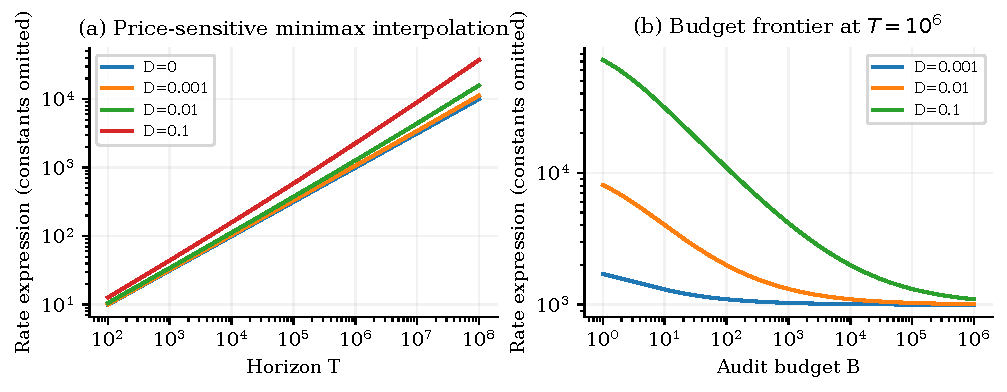
\includegraphics[width=\linewidth]{../figures/06-theory-rates.pdf}
\caption{The proved rate expressions, with universal constants and logarithmic factors omitted. These curves are theoretical illustrations. A positive execution-price spread creates a calibration term; a larger audit budget reduces that term without eliminating ordinary arm exploration.}\label{fig:rates}
\end{figure}

\section{Decision certificates and channel misspecification}
\subsection{A certificate based on the current confidence region}
Let $[\ell,u]\subseteq[\gamma_0,1]$ be a confidence interval for the scale, and let $[\widehat\lambda_i-r_i,\widehat\lambda_i+r_i]$ cover each proxy mean. Certify action $i$ if, for every $j\ne i$,
\begin{equation}
\widehat\lambda_i-r_i-\widehat\lambda_j-r_j-g(c_i-c_j)\geq0
\quad\text{at both }g=\ell,u.
\label{eq:certificate}
\end{equation}
On the joint coverage event this action is truly optimal. The proof is immediate from affine interpolation and~\eqref{eq:identity}. Computing the certificate requires $O(K^2)$ elementary comparisons, or $O(K)$ for a specified candidate. Unlike a plug-in ranking, it exposes whether the decision remains valid over the unresolved calibration range.

For a unique best arm, define its calibration margin
\begin{equation}
\rho=\min_{i:c_i\ne c_{i^*}}
\frac{\gamma\Delta_i}{|c_i-c_{i^*}|},
\label{eq:margin}
\end{equation}
with an empty minimum equal to infinity. If $r_i+r_{i^*}<\gamma\Delta_i/4$ for all $i\ne i^*$ and the scale interval is formed with radius $s<\rho/4$ around an estimate within $s$ of $\gamma$, then~\eqref{eq:certificate} certifies $i^*$. Indeed its left side is at least
$\gamma\Delta_i-2(r_i+r_{i^*})-2s|c_i-c_{i^*}|>0$.
For known proxy means the weaker condition $2s<\rho$ suffices. These are sufficient certificate conditions, not an instance-optimal audit-allocation theorem. Stopping permanently when a certificate holds is valid on simultaneous coverage, but a complete regret analysis of a policy that audits only near unresolved envelope crossings is left open.

\subsection{A quantitative limit on transfer}
Suppose instead that each arm has a stationary binary channel satisfying
\begin{equation}
\left|\Pp(Z=1\mid Y=y,I=i)-\left(\frac{1-\gamma}{2}+\gamma y\right)\right|
\leq\varepsilon\quad (i\in[K],\ y\in\{0,1\}).
\label{eq:misspec}
\end{equation}
Draws are still fresh conditional on the chosen arm. This permits bounded asymmetry and action dependence.
\begin{proposition}[Misspecification penalty]\label{prop:robust}
For $n\geq1$, the bound~\eqref{eq:upper} remains valid after adding
$2(1+D)\varepsilon T/\gamma_0$ to its right-hand side.
\end{proposition}
\begin{proof}
Write $\lambda_i=(1-\gamma)/2+\gamma\mu_i+b_i$ with $|b_i|\leq\varepsilon$. For the signed agreement, conditional on any past history and selected action, its conditional mean differs from $\gamma$ by at most $2\varepsilon$. The bounded martingale version of Hoeffding's inequality gives calibration error at most $2\varepsilon+e_m$ for every positive prefix size $m$; at size zero the bound is still valid. The per-arm proxy concentration is unchanged. Repeating~\eqref{eq:one-step}, its right side gains at most $2\varepsilon$ from $b_i-b_{i^*}$ and $2D\varepsilon$ from calibration bias. Sum, divide by $\gamma_0$, and use the same failure-event bound.
\end{proof}
A small conditional channel error therefore has a potentially linear cumulative consequence. This result is a robustness bound for the stated algorithm, not an impossibility theorem for learners using trusted outcomes to estimate each arm separately.

\section{Numerical study}\label{sec:experiments}
The experiments examine the finite-sample consequences of the model and the conservatism of the proof-oriented policy. They are synthetic Bernoulli simulations, not measurements of an LLM or a production router. All reported outcomes are computed from executed code. The artifact contains the generator, a readable online policy, a separately implemented compiled simulator, per-seed observations, figure scripts, and executable checks.

\paragraph{Protocol.}
We use 256 seeds per environment, audit price $a=0.2$, $\gamma_0=1/4$, and $\delta=T^{-2}$. The principal two-arm family is~\eqref{eq:hardpair} with $h=0.1$, both signs, and $D=0.2$ unless varied. Horizon values are $512,2048,8192,32768$. The default audit budget is $\min\{T,\lceil(DT/a)^{2/3}\rceil\}$, with zero audits for $D=0$; the logarithmic factor is omitted from this practical budget rule, while Theorem~\ref{thm:upper} applies to every budget. Separate sweeps vary the audit budget and execution-price spread. Additional tests vary the number of actions and violate the shared-channel assumption. Parameters were fixed before the simulation outcomes were inspected.

We compare \SC\ with (i) oracle-scale UCB, which knows $\gamma$ and pays no audits; (ii) naive proxy UCB, which subtracts unscaled prices; (iii) rank-only UCB, which ignores prices; (iv) audit-only explore-then-commit (ETC), which distributes the same $B$ audits round-robin, then chooses the largest audited success mean minus price; and (v) audit-all UCB, which observes and uses truth every round. These are transparent information and mechanism controls, not implementations of all algorithms in related work. Every method is charged for its own audits. The first, third, and fourth comparisons deliberately isolate different information assumptions. We report execution regret separately from audit expenditure. The random streams are paired across methods within each environment; seeds are independent within each comparison. Error bars are $1.96$ Monte Carlo standard errors, and do not account for model misspecification.

\begin{table}[t]
\centering\small
\caption{At $T=32768$, $D=0.2$, $h=0.1$, and $a=0.2$, empirical regret over 256 seeds (mean $\pm$ one Monte Carlo standard error). \SC\ and audit-only ETC each use 1024 audits. Oracle-scale UCB receives the true scale. Audit-all UCB pays for 32768 audits.}\label{tab:results}
\begin{tabular}{lrrrr}
\toprule
& \multicolumn{2}{c}{$\gamma=0.4$} & \multicolumn{2}{c}{$\gamma=0.6$} \\
Method & Execution & Total & Execution & Total \\
\midrule
SC-UCB & $401.8\,\pm\,7.2$ & $606.6\,\pm\,7.2$ & $272.6\,\pm\,5.0$ & $477.4\,\pm\,5.0$ \\
Oracle-scale UCB & $404.8\,\pm\,6.0$ & $404.8\,\pm\,6.0$ & $262.3\,\pm\,4.0$ & $262.3\,\pm\,4.0$ \\
Naive proxy UCB & $1582.8\,\pm\,0.9$ & $1582.8\,\pm\,0.9$ & $36.8\,\pm\,0.5$ & $36.8\,\pm\,0.5$ \\
Rank-only UCB & $55.7\,\pm\,0.8$ & $55.7\,\pm\,0.8$ & $1054.3\,\pm\,0.6$ & $1054.3\,\pm\,0.6$ \\
Audit-only ETC & $81.4\,\pm\,18.3$ & $286.2\,\pm\,18.3$ & $194.8\,\pm\,24.8$ & $399.6\,\pm\,24.8$ \\
Audit-all UCB & $155.4\,\pm\,2.3$ & $6709.0\,\pm\,2.3$ & $170.3\,\pm\,2.5$ & $6723.9\,\pm\,2.5$ \\
\bottomrule
\end{tabular}

\end{table}

\paragraph{Identical proxies, opposing decisions.}
Table~\ref{tab:results} and Figure~\ref{fig:horizon} expose the ambiguity directly. The naive proxy policy is favored in the $\gamma=0.6$ world and performs poorly in the $\gamma=0.4$ world; the ranking-only policy exhibits the opposite pattern. Their cheap observations cannot identify which case holds. Calibration substantially improves the unfavorable-world behavior of these policies, but its audit cost is visible. At the largest horizon, \SC\ has total regret about $607$ and $477$ in the two worlds, while audit-only ETC has about $286$ and $400$. Thus the proved algorithm does \emph{not} dominate direct audited learning on these fixed-gap instances. Its large UCB exploration bonuses and explicit audit budget are material costs. This observation is compatible with a minimax theorem, which concerns a supremum over instances, not the best algorithm on one separated pair.

\begin{figure}[t]
\centering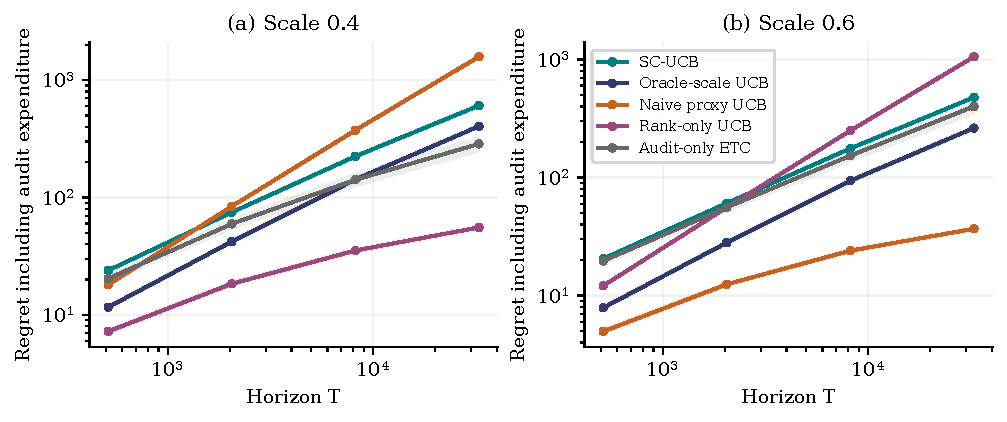
\includegraphics[width=\linewidth]{../figures/02-horizon.pdf}
\caption{Measured total regret for the two indistinguishable-proxy worlds. Shading is $1.96$ Monte Carlo standard errors over 256 paired seeds. Fixed $h=0.1$ does not constitute an empirical estimate of the minimax exponent.}\label{fig:horizon}
\end{figure}

\paragraph{Audits have both value and price.}
Figure~\ref{fig:budget} uses $T=8192$ and seven audit budgets, ranging from zero to the full horizon. Acquiring more trusted labels can reduce execution regret, but paying for every label can dominate the total objective. The two panels must be interpreted together: an audit policy cannot be evaluated from decision error alone. The complete price-spread and action-count sweeps, along with the specification of the stress tests, appear in Appendix~\ref{app:experiments}. In particular, larger $K$ does not make \SC\ free of exploration costs, and action-dependent noise can bias a pooled scale estimate.

\begin{figure}[t]
\centering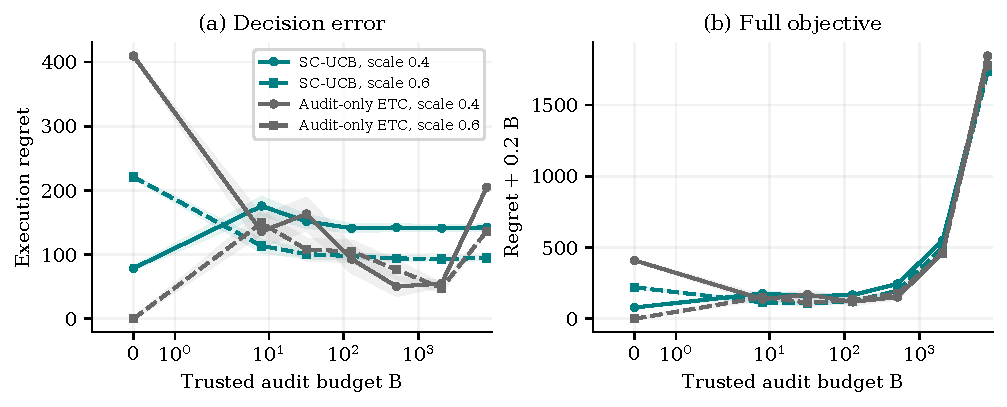
\includegraphics[width=\linewidth]{../figures/03-budget.pdf}
\caption{Budget sweep at $T=8192$. Left: execution regret. Right: the same quantity plus audit expenditure. The same budget is used by both audited policies, including the zero-audit control. Curves distinguish scale $0.4$ (solid) and scale $0.6$ (dashed).}\label{fig:budget}
\end{figure}

\paragraph{Mathematical and implementation checks.}
Exact rational arithmetic verifies the equal-proxy identity and the opposite-sign utility gaps. Grid checks evaluate the full audited joint laws and the KL inequality in both directions. Additional tests check certificate soundness, signed-agreement expectations, the audit budget, and a feedback interface that rejects access to unaudited truth. The readable policy and compiled simulator agree on an independently replayed trajectory. These checks detect implementation and algebraic errors; the theorem proofs, not numerical agreement, justify the bounds.

\section{Discussion}
The results suggest a specific design principle for paid tool selection: evaluate whether an automatic score preserves the \emph{price-adjusted} decision over plausible calibrations, rather than checking quality ranking alone. A trusted test execution can calibrate future decisions across tools when the shared-channel condition is justified. The endpoint certificate provides a small implementable component for exposing whether a decision still depends on unresolved evaluator reliability. These are potential applications to monitoring and routing; monetary savings, latency improvements, and validity for any particular language-model judge are not established here.

Several restrictions matter. The analysis is stochastic and stationary; tool prices are known and fixed; the main channel is symmetric and shared; trusted audits are correct; and the audited outcome is available after the decision. An audit which repairs the current action, an action-dependent evaluator, correlated temporal errors, or unknown prices changes the problem. The robustness proposition quantifies only bounded deviations from the channel, not arbitrary evaluator behavior. The lower bounds are sharp in $T,B,D,a$ up to logarithms for two arms and a fixed reliability floor. General-$K$ lower bounds, adaptation to unknown horizons and price geometry with sharper constants, and decision-triggered audit schedules are further questions.

The central conclusion is that positive ranking information and cost-sensitive decision information are different resources. In this model, their difference is a shared scalar, but learning that scalar has a provable audit cost that varies continuously with execution-price heterogeneity.

\bibliography{references}

\appendix
\section{Additional experimental details and results}\label{app:experiments}
\paragraph{Generation and accounting.}
The release includes 46 parameter configurations and six policies, with the oracle-scale policy omitted in the four nonzero misspecification configurations because there is no shared oracle scale there. This yields 69,632 policy--environment--seed runs, each recorded at one-quarter, one-half, and the final horizon: 208,896 rows. Different configurations reuse seed labels; the total run count must not be interpreted as 69,632 independent experimental units for a pooled significance test. Within a configuration, 256 random streams are independent and shared across policy comparisons. Each round draws one uniform variate for true success and one for the proxy conditional on that success. The number of random draws does not depend on auditing. The simulator computes realized action-wise pseudo-regret from known generating means, rather than subtracting two noisy reward sums.

\paragraph{Action-count sweep.}
At $T=8192$, $D=0.2$, and $\gamma=0.4$, the $K=2$ point uses the principal pair. For $K\in\{4,8,16,32\}$, prices are equally spaced in $[0,D]$, and means are $\mu_i=0.5+c_i+d_i$ with $d_i$ equally spaced from $-0.06$ to $0.06$. The utility gaps therefore change with $K$; this is a family of instances, not a controlled experiment varying only cardinality. The same budget rule is used at every $K$. Figure~\ref{fig:stress}(a) shows that the calibration-sharing interpretation does not remove the costs of exploring many arms.

\paragraph{Misspecification sweep.}
At $T=8192$, $D=0.2$, $h=0.1$, and sign $-$, start with the nominal false-positive and false-negative probabilities $0.3$. For $\varepsilon\in\{0,0.03,0.06,0.12,0.2\}$, subtract $\varepsilon$ from both error probabilities of action 0 and add it to both error probabilities of action 1. These valid conditional probabilities differ from the nominal channel by at most $\varepsilon$ as in~\eqref{eq:misspec}. Means, prices, and the audit budget remain fixed. Figure~\ref{fig:stress}(b) reports the resulting regret. This is an assumption stress test and is not an estimate of evaluator bias in deployed systems.

\begin{figure}[ht]
\centering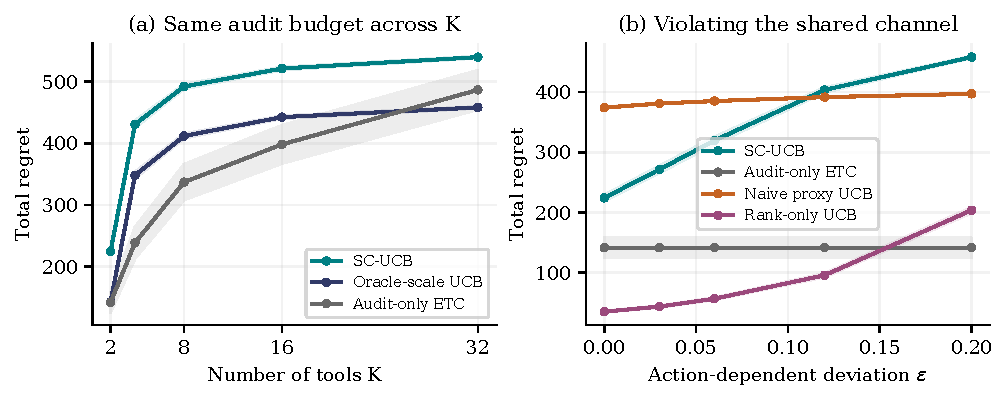
\includegraphics[width=\linewidth]{../figures/04-structure-stress.pdf}
\caption{Additional mechanism checks. Left: a family with varying $K$ and the same audit budget. Right: deliberate action-dependent channel deviations. The oracle-scale control is excluded when no shared scale exists.}\label{fig:stress}
\end{figure}
\begin{figure}[ht]
\centering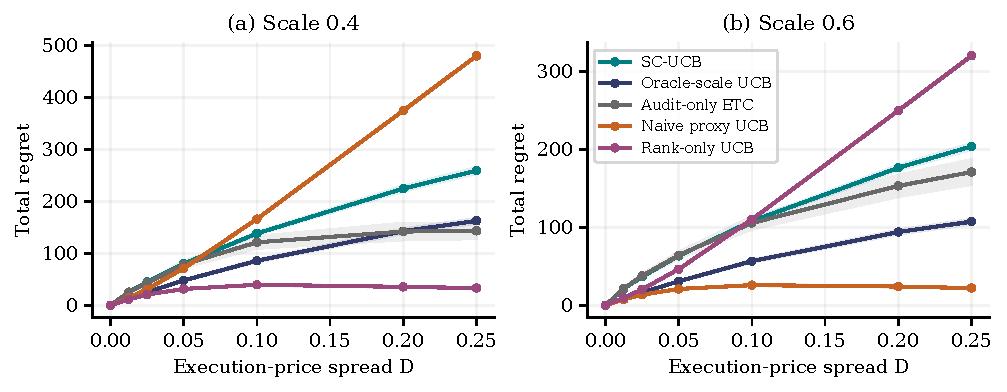
\includegraphics[width=\linewidth]{../figures/05-spread.pdf}
\caption{Price-spread sweep at $T=8192$ in both worlds of~\eqref{eq:hardpair}. Changing $D$ changes both true quality gaps and execution-price gaps while preserving the paired-world proxy identity. At $D=0$ the two actions in this particular family have equal quality as well as equal price, so zero regret here is not a test of the general equal-price $\sqrt T$ lower bound.}\label{fig:spread}
\end{figure}

\section{Reproducibility and further verification}\label{app:reproduce}
The Python package exposes a feedback-restricted online interface: \texttt{choose()} returns an action and an audit request, and \texttt{update(proxy, truth)} accepts a truth value only on audited rounds. Environment construction and regret evaluation live outside this interface. The experimental simulator has access to latent outcomes to score performance, while action selection uses only the designated observations.

From a clean checkout, create a Python environment, install \texttt{requirements-lock.txt}, run the test suite with \texttt{python -m pytest -q}. The two experiment scripts are:
\begin{verbatim}
python scripts/run_experiments.py
python scripts/analyze.py
\end{verbatim} The experimental manifest records the configurations, seed range, elapsed time, and SHA-256 hash of the raw results. The analysis script generates all tables and figures from the retained runs. The paper is built with the official ALT 2027 template. \providecommand{\artifactlocation}{The reference implementation is included in Appendix~\ref{app:code}; author-identifying repository links are omitted for review.}\artifactlocation

For direct verification of Lemma~\ref{lem:kl}, the audited probability vector, in lexicographic order on the binary pair $(Y,Z)$, is
\begin{equation}
\left((1-\mu)\frac{1+\gamma}{2},\ (1-\mu)\frac{1-\gamma}{2},\ \mu\frac{1-\gamma}{2},\ \mu\frac{1+\gamma}{2}\right).
\end{equation}
Summing entries with $Z=1$ recovers~\eqref{eq:identity}; weighting entries by $(1,-1,-1,1)$ gives~\eqref{eq:agreement}. This explicit law is also used by the numerical KL checks. A confidence certificate is verified against dense scale grids and extreme proxy-interval values, independently of the endpoint implementation. Those finite checks are supplementary to the affine proof and do not replace it.

\clearpage
\section{Reference online implementation}\label{app:code}
The following executable NumPy implementation is the policy used in the replay check. It accepts only the observations specified by the protocol. In a deployment, the caller supplies a trusted outcome precisely when \texttt{choose()} requests an audit. The compiled simulator used for the larger study is verified against this interface at zero, partial, and full audit budgets.
\lstinputlisting[lastline=47,basicstyle=\ttfamily\fontsize{9}{9.5}\selectfont]{../src/auditband/policy.py}
\end{document}
